\documentclass[a0paper,portrait]{baposter}
\usepackage{wrapfig}
\usepackage{lmodern}
\usepackage{enumerate}
\usepackage[utf8]{inputenc} %unicode support
\usepackage[T1]{fontenc}
\usepackage{amssymb,amsfonts,amsmath,mathtext,enumerate,float}


\selectcolormodel{cmyk}
\graphicspath{{fig/}} % Directory in which figures are stored
\newcommand{\compresslist}{%
\setlength{\itemsep}{0pt}%
\setlength{\parskip}{1pt}%
\setlength{\parsep}{0pt}%
}

\DeclareMathOperator*{\indicator}{\mathds{1}}
\DeclareMathOperator*{\softmax}{softmax}
\DeclareMathOperator*{\idx}{idx}
\DeclareMathOperator*{\pos}{pos}
\DeclareMathOperator*{\AUCH}{AUCH}
\DeclareMathOperator*{\tf}{tf}
\DeclareMathOperator*{\ntf}{ntf}
\DeclareMathOperator*{\idf}{idf}
\DeclareMathOperator*{\ndf}{ndf}
\DeclareMathOperator*{\similarity}{sim}
\DeclareMathOperator*{\argmin}{arg\,min}
\DeclareMathOperator*{\const}{const}
\DeclareMathOperator*{\dBeta}{Beta}
\DeclareMathOperator*{\dDir}{Dir}
\DeclareMathOperator*{\Tr}{Tr}
\DeclareMathOperator*{\dDP}{DP}
\DeclareMathOperator*{\dMult}{Mult}
\DeclareMathOperator*{\dBern}{Bern}
\DeclareMathOperator*{\dCRP}{CRP}
\DeclareMathOperator*{\dKL}{KL}
\DeclareMathOperator*{\diag}{diag}

\newcommand{\dd}[1]{\mathrm{d}{#1}}
\newcommand{\avep}{\mathrm{AveP}}
\newcommand{\precision}{p@k}
\newcommand{\dcg}{\mathrm{DCG}}
\newcommand{\rel}{\mathrm{rel}}

% BOLD
\newcommand{\bmatr}{{\mathbf{B}}}
\newcommand{\cmatr}{{\mathbf{C}}}
\newcommand{\hmatr}{{\mathbf{H}}}
\newcommand{\fmatr}{{\mathbf{F}}}
\newcommand{\mmatr}{{\mathbf{M}}}
\newcommand{\xmatr}{{\mathbf{X}}}
\newcommand{\pmatr}{{\mathbf{P}}}
\newcommand{\xmatrt}{{\tilde{\mathbf{X}}}}
\newcommand{\imatr}{{\mathbf{I}}}
\newcommand{\vmatr}{{\mathbf{V}}}
\newcommand{\wmatr}{{\mathbf{W}}}
\newcommand{\umatr}{{\mathbf{U}}}
\newcommand{\zmatr}{{\mathbf{Z}}}
\newcommand{\zmatrt}{{\tilde{\mathbf{Z}}}}
\newcommand{\Tmatr}{\mathbf{T}}
\newcommand{\lambdamatr}{{\mathbf{\Lambda}}}
\newcommand{\phimatr}{\mathbf{\Phi}}
\newcommand{\sigmamatr}{\mathbf{\Sigma}}
\newcommand{\thetamatr}{\boldsymbol{\Theta}}

\newcommand{\ab}{{\mathbf{a}}}
\newcommand{\bb}{{\mathbf{b}}}
\newcommand{\cb}{{\mathbf{c}}}
\newcommand{\db}{{\mathbf{d}}}
\newcommand{\eb}{{\mathbf{e}}}
\newcommand{\fb}{{\mathbf{f}}}
\newcommand{\gb}{{\mathbf{g}}}
\newcommand{\hb}{{\mathbf{h}}}
\newcommand{\mb}{{\mathbf{m}}}
\newcommand{\pb}{{\mathbf{p}}}
\newcommand{\qb}{{\mathbf{q}}}
\newcommand{\rb}{{\mathbf{r}}}
\newcommand{\tb}{{\mathbf{t}}}
\newcommand{\ub}{{\mathbf{u}}}
\newcommand{\vb}{{\mathbf{v}}}
\newcommand{\wb}{{\mathbf{w}}}
\newcommand{\xb}{{\mathbf{x}}}
\newcommand{\xt}{{\tilde{x}}}
\newcommand{\xbt}{\tilde{{\mathbf{x}}}}
\newcommand{\yb}{{\mathbf{y}}}
\newcommand{\zb}{{\mathbf{z}}}
\newcommand{\zt}{{\tilde{z}}}
\newcommand{\zbt}{{\tilde{\mathbf{z}}}}
\newcommand{\mub}{{\boldsymbol{\mu}}}
\newcommand{\alphab}{{\boldsymbol{\alpha}}}
\newcommand{\thetab}{\boldsymbol{\theta}}
\newcommand{\iotab}{\boldsymbol{\iota}}
\newcommand{\zetab}{\boldsymbol{\zeta}}
\newcommand{\xib}{\boldsymbol{\xi}}
\newcommand{\xibt}{\tilde{\boldsymbol{\xi}}}
\newcommand{\xit}{\tilde{\xi}}
\newcommand{\betab}{{\boldsymbol{\beta}}}
\newcommand{\phib}{{\boldsymbol{\phi}}}
\newcommand{\psib}{{\boldsymbol{\psi}}}
\newcommand{\gammab}{{\boldsymbol{\gamma}}}
\newcommand{\lambdab}{{\boldsymbol{\lambda}}}
\newcommand{\varepsilonb}{{\boldsymbol{\varepsilon}}}
\newcommand{\pib}{{\boldsymbol{\pi}}}

\newcommand{\scl}{s_{\mathsf{c}}}
\newcommand{\shi}{s_{\mathsf{h}}}
\newcommand{\shib}{\mathbf{s}_{\mathsf{h}}}
\newcommand{\MOD}{M}
\newcommand{\entr}{\mathsf{H}}
\newcommand{\REG}{\Omega}
\newcommand{\Mquol}{V}
%\newcommand{\prob}{\mathsf{P}}
\newcommand{\prob}{p}
\newcommand{\expec}{\mathsf{E}}

% overline
\newcommand{\xo}{{\overline{x}}}
\newcommand{\yo}{{\overline{y}}}

% bold overline
\newcommand{\xbo}{{\overline{\mathbf{x}}}}

\newcommand{\Amc}{{\mathcal{A}}}
\newcommand{\Bmc}{{\mathcal{B}}}
\newcommand{\Cmc}{{\mathcal{C}}}
\newcommand{\Jmc}{{\mathcal{J}}}
\newcommand{\Imc}{{\mathcal{I}}}
\newcommand{\Kmc}{{\mathcal{K}}}
\newcommand{\Lmc}{{\mathcal{L}}}
\newcommand{\Mmc}{{\mathcal{M}}}
\newcommand{\Nmc}{{\mathcal{N}}}
\newcommand{\Pmc}{{\mathcal{P}}}
\newcommand{\Tmc}{{\mathcal{T}}}
\newcommand{\Vmc}{{\mathcal{V}}}
\newcommand{\Wmc}{{\mathcal{W}}}

\newcommand{\T}{^{\text{\tiny\sffamily\upshape\mdseries T}}}
\newcommand{\deist}{\mathbb{R}}
\newcommand{\ebb}{\mathbb{E}}

%ALEX
\newcommand{\Amatr}{\mathbf{A}}
\newcommand{\X}{\mathbf{X}}
\newcommand{\Z}{\mathbf{Z}}
\newcommand{\Umatr}{\mathbf{U}}
\newcommand{\zetavec}{\boldsymbol{\zeta}}

\newcommand{\M}{\mathbf{M}}
\newcommand{\x}{{\mathbf{x}}}
\newcommand{\z}{{\mathbf{z}}}
\newcommand{\ical}{{\mathcal{I}}}
\newcommand{\tvec}{{\mathbf{t}}}
\newcommand{\xvec}{{\mathbf{x}}}
\newcommand{\zvec}{{\mathbf{z}}}
\newcommand{\bvec}{{\mathbf{b}}}
\newcommand{\qvec}{{\mathbf{z}}}
\newcommand{\pvec}{{\mathbf{p}}}
\newcommand{\wvec}{{\mathbf{w}}}
\newcommand{\rvec}{{\mathbf{r}}}
\newcommand{\thetavec}{{\mathbf{\theta}}}
\newcommand{\y}{{\mathbf{y}}}
\newcommand{\g}{{\mathbf{g}}}
\newcommand{\w}{{\mathbf{w}}}
\newcommand{\m}{{\mathbf{m}}}
\DeclareMathOperator*{\argmax}{arg\,max}



\newenvironment{boenumerate}
  {\begin{enumerate}\renewcommand\labelenumi{\textbf\theenumi.}}
  {\end{enumerate}}
\begin{document}

\definecolor{darkgreen}{cmyk}{1,1,0,0.455}
\definecolor{lightgreen}{cmyk}{1,1,0,0.455}

\begin{poster}
{
grid=false,
headerborder=open, % Adds a border around the header of content boxes
colspacing=1em, % Column spacing
bgColorOne=white, % Background color for the gradient on the left side of the poster
bgColorTwo=white, % Background color for the gradient on the right side of the poster
borderColor=darkgreen, % Border color
headerColorOne=lightgreen, % Background color for the header in the content boxes (left side)
headerColorTwo=lightgreen, % Background color for the header in the content boxes (right side)
headerFontColor=white, % Text color for the header text in the content boxes
boxColorOne=white, % Background color of the content boxes
textborder=rounded, %rectangle, % Format of the border around content boxes, can be: none, bars, coils, triangles, rectangle, rounded, roundedsmall, roundedright or faded
eyecatcher=false, % Set to false for ignoring the left logo in the title and move the title left
headerheight=0.11\textheight, % Height of the header
headershape=rounded, % Specify the rounded corner in the content box headers, can be: rectangle, small-rounded, roundedright, roundedleft or rounded
headershade=plain,
headerfont=\Large\textsf, % Large, bold and sans serif font in the headers of content boxes
%textfont={\setlength{\parindent}{1.5em}}, % Uncomment for paragraph indentation
linewidth=2pt % Width of the border lines around content boxes
}
{}
%
%----------------------------------------------------------------------------------------
%	TITLE AND AUTHOR NAME
%----------------------------------------------------------------------------------------
%
{
\textsf %Sans Serif
{Hierarchical Thematic Classification of Major~Conference~Proceedings
}
}            
{\sf\vspace{0.2em}\\
Arsentii Kuzmin, Alexander Aduenko, and Vadim Strijov 
\vspace{0.1em}\\
\small{ Moscow Institute of Physics and Technology --- 
Laboratory of Machine Intelligence\\
\vspace{0.2em}\\
strijov@phystech.edu}
}
{\includegraphics[width=.22\textheight]{eng_text}} % University logo

\headerbox{Hierarchical text classification
}{name=one_left,column=0,row=0, span=1}{
The thematic model of a text collection is a map, which determines a set of topics from some given hierarchical structure of topics for each document from the collection. The text collections are abstracts of conference proceedings, or text messages from social networks, or research papers. The thematic model assists in searching through collections efficiently. However the model construction is often labour-intensive. Some collections already have their structure and subset of documents, which have been partially classified by experts. To simplify the classification procedure the authors propose an algorithm to rank topics for a given document in a collection~\cite{Alexandrov,Joahims}. 
}

\headerbox{EURO conference thematic modelling}{name=one_right,column=1,row=0, span=2}{
\begin{minipage}{0.66\textwidth}
Every year the program committee the  European Conference on Operational Research~(EURO) builds a schedule (thematic model) for this conference using a set of submitted abstracts.
The structure of this model consists of~$26$ major areas. Each Area consists of~$10-15$ streams. Each stream consists of~$5-10$ Sessions. Each session consists of four talks in a row. The participants submit short abstracts to the program committee to proceed. 
There are two types of participants: invited participants and new, contributed, participants. The invited participants already have a determined session, so the collection of abstracts is partly labelled.
For each contributed participant, the program committee should select the most relevant session according to the content of the abstract and according to the conference structure. The program committee invites up to~$200$ experts from  different research areas to construct the thematic model.
\end{minipage}
\begin{minipage}{0.34\textwidth}
    \includegraphics[width=\linewidth]{euro_start.png} 
\end{minipage}
}

\headerbox{Hierarchical similarity function}{name=two_left,column=0,below=one_left,span=2}{
We propose a weighted hierarchical similarity function to calculate the topic relevance. The function calculates the similarity of a document and a tree branch. The weights in this function determine word importance. We use the entropy of words to estimate the weights~\cite{Kuznetsov,Tokmakova}. 

\bigskip
\textbf{The weighted similarity} of the document~$\xb$ and the cluster~$c_{\ell, k}$
%\[
$s(\xb,\:c_{\ell, k}) = \xb\T \lambdamatr \mub(c_{\ell, k}),$ 
%\]
%\vspace{-0.1cm}
where~$\lambdamatr = \diag(\lambda_1, \cdots, \lambda_{|W|})$ is the word importance matrix, and~$\lambda_i$ is the importance of the word~$w_i$.

\bigskip
\begin{minipage}[h]{0.5\textwidth}
\vspace{-4pt}
    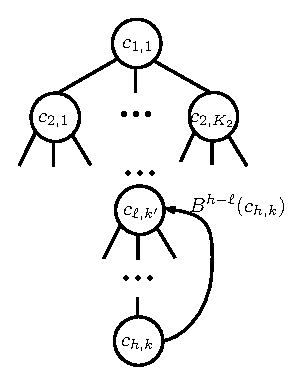
\includegraphics[width=0.39\textwidth]{hierarchy_start.eps}
    \includegraphics[width=0.49\textwidth]{theta_params.eps}\\
    \vspace{-2pt}
    {\small{Cluster hierarchy~~~Cluster branch~$c_{h, k}$, weights}}
\end{minipage}
\begin{minipage}[h]{0.5\textwidth}
\textbf{The hierarchical similarity function}  of the document~$\xb$ and the cluster~$c_{h, k}$ is $s_{\mathsf{h}}(\xb_n,\: c_{h,\,k}) =$
\[
 =\sum_{\ell = 1}^{h} \theta_{k}^{\ell} s\bigl(\xb_n,\:B^{h - \ell}(c_{h,\,k})\bigr) = \xb_n\T \lambdamatr \mmatr_k \thetab_k,
\]
where~$\theta^{\ell}_k$ weight of the cluster of level~$\ell$ on the branch~$k$, and~$\mmatr_k$~--~matrix of centers of parent clusters~$c_{h,k}$:
\[
\mub_{\ell,k} = \mub\bigl( B^{h-\ell}(c_{h,k})\bigr), \quad \mmatr_k = [\mub_{1,k}, \dots, \mub_{h,k}].
\]
\end{minipage}
}

\headerbox{Hierarchical ranking quality}{name=physical,span=1,column=2,below=one_left}{ 
We introduce the ranking operator $R: \:\deist^{|W|} \to S^{K_h}$. It maps the document~$\xb \in \deist^{|W|}$ to the permutation $q(\xb) \in S^{K_h}$ of the clusters~$\{h\}$.
\vspace{-1.1cm}
\center{
\includegraphics[width=0.75\textwidth]{AUC_example.eps}
}
\vspace{-0.4cm}
\[
\text{Hist}(k) = \#\{n: \; \mathrm{pos}\bigl(R(\xb_n),\,c(\xb_n)\bigr) \leq k\},
\]
\vspace{-0.7cm}
\[
\AUCH(R) = \dfrac{1}{k_h |D|}\sum_{k=1}^{k_h}{\text{Hist}(k)}.
\]
}

\headerbox{Joint model of document clusters}{name=three_left,column=0,below=two_left,span=1}{
The probability of some document~$\xb_n$ belongs some cluster~$c_{h, k}$ is
\vspace{-0.2cm}
\[
p(\xb_n \in c_{h,k} |\thetab, \alphab) =  \softmax(\shib(\xb_n | \thetab_k, \alphab))_k.
\]
\vspace{-0.1cm}
\textbf{The probabilistic model} $p(\zmatr,\thetab, \mb, \vmatr, \alphab)$ of the document classes~$\zmatr$, $z_{nk} = 1$ for $\xb_{n}$ belong $c_{h, k}$ is
\vspace{-0.2cm}
\[
p(\zmatr,\thetab, \mb, \vmatr, \alphab) = L(\zmatr | \thetab, \alphab)\Nmc(\alphab| \mathbf{0}, a^{-1}\imatr)\times
\]
\vspace{-0.2cm}
\[
\times\prod_k \Nmc(\thetab_k| \mb_k, \vmatr_k^{-1})\Nmc\Wmc(\mb_k, \vmatr_k | \mb_0, b, \wmatr, \nu).
\]

\textbf{The probability estimate} of some \emph{\color{red}unclassified} document $\xbt_t$ belongs some cluster~$c_{h,k}$:\\
\vspace{-0.1cm}
the MAP estimates
\vspace{-0.2cm}
\[p({\color{red}\zt_{tk}}|\xbt_t) = p({\color{red}\zt_{tk}}|\xbt_t, \thetab_k^{\text{MAP}}, \alphab^{\text{MAP}}),\]
\vspace{-0.2cm}
the evidence estimates 
\vspace{-0.2cm}
\[p({\color{red}\zt_{tk}}|\xbt_t) = \int p({\color{red}\zt_{tk}} |\xbt_t, \thetab, \alphab ) p(\thetab, \alphab| \zmatr) \dd \thetab \dd \alphab.\]
}

\headerbox{Ranking results of hierarchical similarity function}{name=three_right,span=2,column=1,below=two_left}{ 
For the ranking experiment, we considered the area and the stream levels of the conferece hierarchy. We constructed the ranking operator~$R$ using the proposed weighted hierarchical similarity function hSim and used the EM algorithm to optimize its parameters on the training subset. The results of this function were compared with results several algorithms of hierarchical ranking: 1)~the hierarchical naive Bayes hNB, 2)~the probabilistic regularized model SuhiPLSA and 3)~the hierarchical multi-class~SVM.

\vspace{0.1cm}
\begin{minipage}[h]{0.4\textwidth}
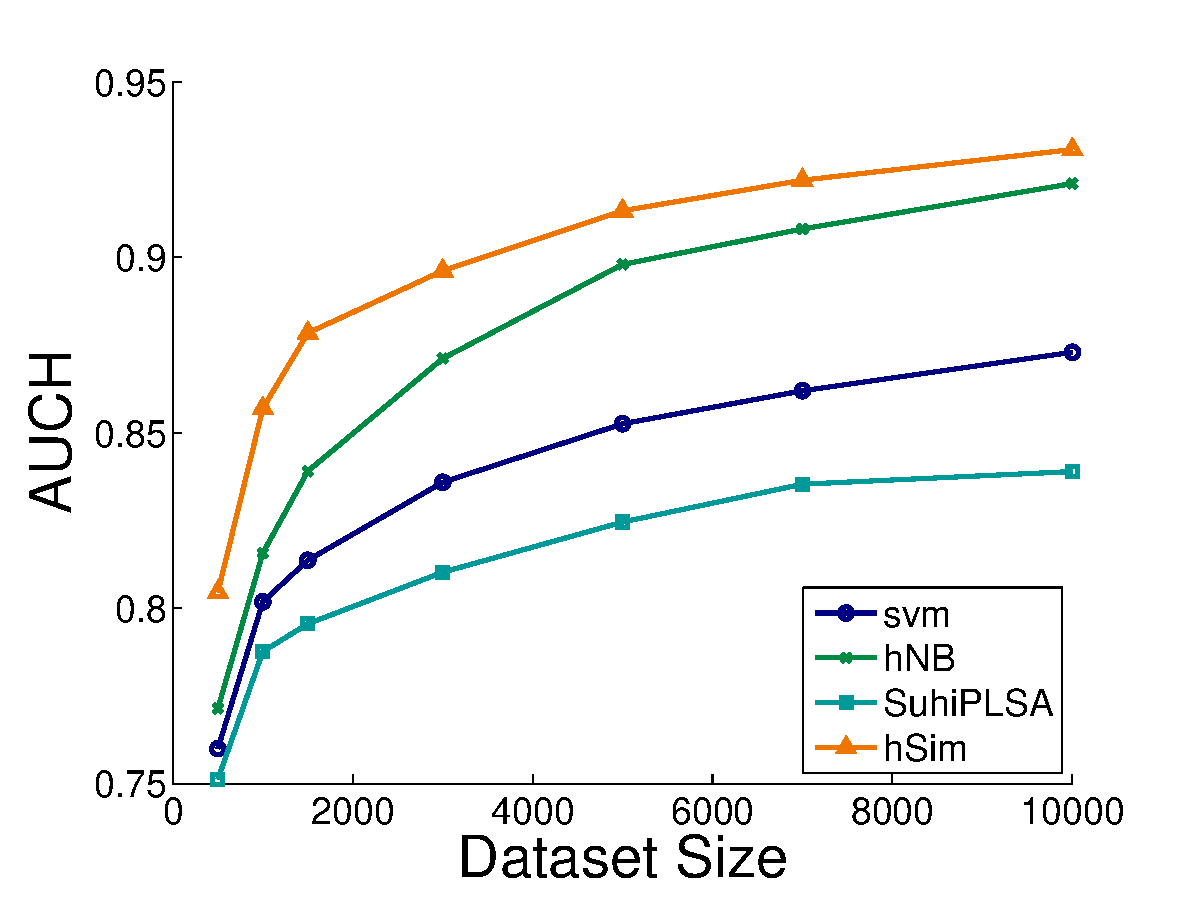
\includegraphics[width=\textwidth]{euro_results_data_size.eps}
Test AUCH quality dependence \\on the training sample size
\end{minipage}
\begin{minipage}[h]{0.6\textwidth}
    \begin{minipage}[h]{0.49\linewidth}
        \includegraphics[width=\textwidth]{area_sim.png}
        Same importance for all words, $\lambdamatr = \imatr$
    \end{minipage}
    \begin{minipage}[h]{0.49\linewidth}
        \includegraphics[width=0.95\textwidth]{area_sim_optimized.png} \\
        Optimized importance of words, $\lambdamatr = \lambdamatr^*$.
    \end{minipage}
\end{minipage}
}

\headerbox{References}{name=references,column=0,span=3,below=three_left}{
{\footnotesize
\renewcommand{\baselinestretch}{0.6}% Reduce the font size in this block
\renewcommand{\section}[2]{\vskip 0.05em} % Get rid of the default "References" section title
\nocite{*} % Insert publications even if they are not cited in the poster
\bibliographystyle{unsrt}
\bibliography{Kuzmin2019Poster} % Use sample.bib as the bibliography file
}}



  
\end{poster}
\end{document}
